\def \eng #1{\foreignlanguage{english}{#1}}
\def \engtt #1{\eng{\texttt{\justify #1}}}

\textbf{Цель работы.} Изучение принципов построения, функционирования и программирования магистрально-модульной аппаратуры КАМАК на примере программно-аппаратной реализации автоматических измерений выходных статических характеристик биполярных транзисторов.

\textbf{Аппаратура.} Лабораторный макет \enquote{биполярных транзистор}, источник питания, аппаратура КАМАК, соединительный кабель, персональный компьютер.

\textbf{Содержание работы.} Снятие выходной статической характеристики биполярного транзистора с использованием аппаратуры КАМАК.

\section{Минимальные теоретические сведения}

\subsection{Статические характеристики транзистора}

Статическими характеристиками транзистора называются зависимости между постоянными токами и напряжениями в его входных и выходных цепях. Совокупность статических характеристик при различных значениях их параметров называется семейством характеристик. Величина, поддерживаемая постоянной при измерении одной характеристики, называется параметром характеристики.

Статической выходной характеристикой транзистора является зависимость выходного тока $I_\text{вых}$ от величины выходного напряжения $U_\text{вых}$ при постоянном значении входного тока $I_\text{вх}$:
%
\begin{equation*}
    I_\text{вых} = f(U_\text{вых})_{I_\text{вх} = \mathrm{const}} .
\end{equation*}
%
Параметром выходной характеристики является входной ток.

Одной из задач экспериментатора, при построении семейств статических характеристик транзистора по экспериментальным данным, является обеспечение постоянства параметра характеристики на всем протяжении измерения. Эта задача осложняется тем, что транзистор~--- нелинейный элемент и, в общем случае, все входные и выходные токи и напряжения зависят друг от друга. Следовательно, значение параметра семейства может варьироваться в зависимости от значения независимой переменной. Это означает, что необходимо контролировать параметр характеристики при изменении значения независимой переменной и регулировкой подаваемого на вход/выход тока/напряжения компенсировать отклонения значения параметра от постоянного значения. Если отклонения значения параметра характеристики на всем протяжении измерения не превышают $3\%-5\%$, то контроль и регулировку параметра можно исключить.

\subsection{Принципиальная схема включения транзистора для измерения выходных статических характеристик}

На \autoref{fig:maket_scheme} представлена принципиальная схема для проведения эксперимента по снятию выходных статических характеристик биполярного транзистора.

\begin{figure}[h]%
    \centering
    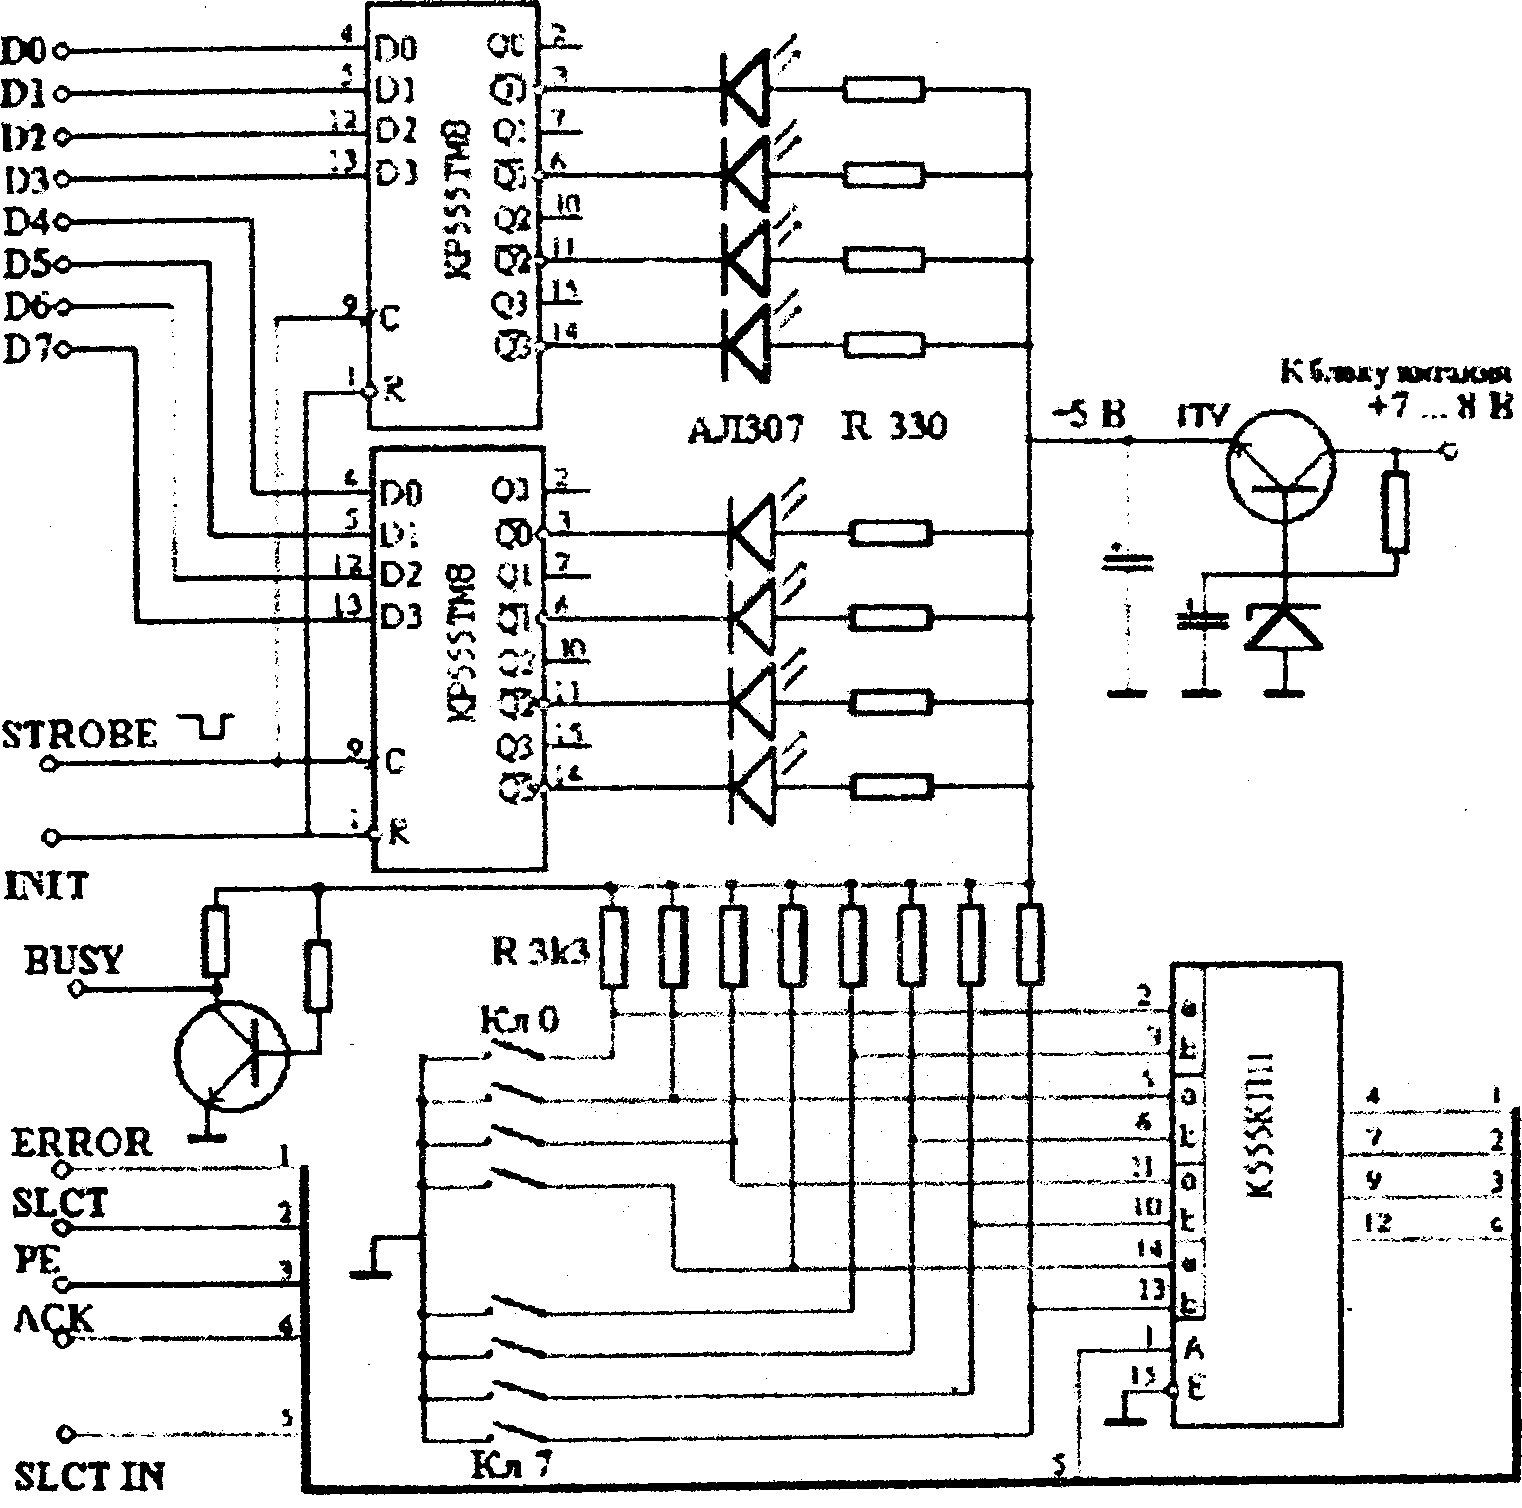
\includegraphics[width=0.5\textwidth]{maket_scheme}%
    \caption[]{Схема включения транзистора для измерения выходных характеристик}%
    \label{fig:maket_scheme}%
\end{figure}

Из-за специфики автоматизированных измерений, отсутствует возможность непосредственного измерения токов в цепи. Поэтому, в схему введены резисторы $R_3$ и $R_4$. Если измерить падение напряжения на этих резисторах то, зная их сопротивления, можно вычислить протекающий через них ток, т.е. получить значения базового и коллекторного токов:
%
\begin{equation*}
    I_\text{вх} = \frac{U_1 - U_\text{вх}}{R_3}, \quad
    I_\text{вых} = \frac{U_2 - U_\text{вых}}{R_4} .
\end{equation*}

Так как измерения производятся в статическом режиме, то необходимо шунтирование возможной переменной составляющей входного напряжения. Для этого в схему введен конденсатор $C_1$.

\subsection{Методика проведения измерений}

Автоматизированное измерение входных и выходных статических характеристик производится с помощью магистрально-модульного измерительного комплекса КАМАК, персональною компьютера типа \eng{IBM PC} и интерфейсной платы-моста \eng{PC}-КАМАК. В крейт КАМАКа установлены модули: крейт-контроллер СМ-ЭВМ, устройство аналоговое запоминающее 16-ти канальное ФК-75, аналогово-цифровой преобразователь ФК71-2 или АЦП-14, 2-х канальный цифро-аналоговый преобразователь 2ЦАП-10.

Модуль ФК-75 запоминает одновременно 16 значений аналогового напряжения на своих 16 входах (предварительно модуль необходимо перевести в режим слежения). В последствии, запомненные значения напряжений могут быть выборочно или последовательно коммутированы на единственный выход модуля. Все входы имеют общую точку. В данной работе используются только 4 канала из 16. Входы подключаются к тем точкам, где необходимо измерить напряжения.

Напряжение с выхода ФК-75 подается на вход АЦП, где и происходит его оцифровка.

Модуль 2ЦАП-10 имеет 2 выхода, на которых можно получить значение напряжения от $0.005$ вольт до $5$ вольт. Необходимое значение напряжения на выходах модуля достигается записью в модуль по одному из субадресов соответствующего числового кода. С выходов 2ЦАП-10 можно задавать базовый ток и напряжение на коллекторе транзистора.

Процедура получения семейства выходных характеристик заключается в следующем:
%
\begin{enumerate}
    \item с помощью одного из выходов 2ЦАП-10 задается некоторое значение параметра семейства $I_\text{вх}$,
    \item с помощью другого выхода 2ЦАП-10 изменяется значение независимом переменной ($U_\text{вых}$ с некоторым шагом (от минимального значения до максимального),
    \item после каждого изменения значения независимой переменной с помощью цепочки модулей ФК-75~-- АЦП снимаются значения напряжений, позволяющие вычислить значение $I_\text{вых}$, которые заносятся в память ЭВМ.
\end{enumerate}

\section{Результаты и их обсуждение}

\subsection{Интерфейс программы управления}

Для организации работы с устройством была разработана программа с графическим интерфейсом (\autoref{fig:app}).

\begin{figure}[h]%
\centering
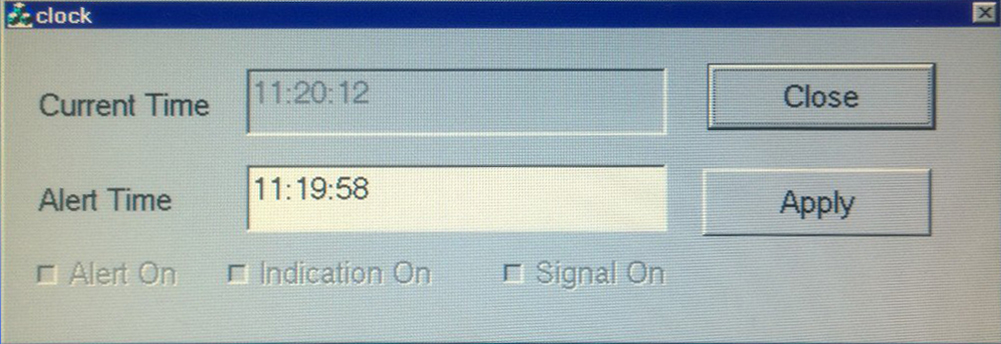
\includegraphics[width=0.5\textwidth]{app}%
\caption[]{Главное окно программы}%
\label{fig:app}%
\end{figure}

Программа по команде оператора в фоновом режиме производит измерение семейства выходных характеристик транзистора в соответствии с указанными при запуске параметрами.

Операторский интерфейс программы предусматривает возможность установить минимальное и максимальное значение параметра и независимой переменной, количество шагов по независимой переменной, а также число характеристик в семействе.

\subsection{Архитектура программы управления}

Программа управления была написана в среде \eng{Microsoft Visual Studio 6.0} на языке \engtt{c++} с использованием библиотеки классов \eng{MFC} (\eng{Microsoft Foundation Classes}).

Для инкапсуляции низкоуровневого программного интерфейса устройства был описан и реализован интерфейс (абстрактный класс) \engtt{CDevice}. Он инкапсулирует процесс снятия выходной характеристики транзистора при заданном значении параметра, выполняющийся в фоновом режиме.

При запуске процесса снятия характеристики метод интерфейса получает на вход функцию обратного вызова, через которую осуществляет информирование инициатора операции о ее готовности.

Результаты измерений выводятся на экран по мере их готовности. Примеры полученных результатов изображены на \autoref{fig:app}.

\section{Выводы}

В ходе работы была реализована программа для автоматизации процесса снятия семейства выходных статических характеристик биполярного транзистора.

Были изучены принципы построения, функционирования и программирования магистрально-модульной аппаратуры КАМАК.
